\chapter{Hierarchical stochastic block model}\label{app:hsbm}
The algorithm called hierarchic Stochastic Block Model (hSBM) from~\cite{gerlach2018network} is hereby summed up.

The first step of hierarchical stochastic block model, as discussed in~\cite{peixoto2014efficient}, is to create a bipartite network $G$ with two kinds of nodes: \textbf{words} and \textbf{documents}. Every time a word $w$ is present in a document $d$ an edge $e_{wd}$ is created. If a word count in the entire corpus is under a certain threshold, that word could be ignored; this is not done in this work. The aim is to find a partition $b\in\{b_i\}$ with $B=\left|\{b_i\}\right|$ blocks.

This model belongs to the so called \textit{generative models}: given the data, the model should generate a network $G$ with probability $P(G|\theta, b)$, where $b$ is the partition and $\theta$ any additional parameter of the model.

Using the well-known Bayes theorem one could estimate the probability that an
observed network was generated by the partition $b$:
\begin{equation}\label{eq:PbonG}
  P(b,\theta|G)=\frac{P(G|b,\theta)\overbrace{P(b,\theta)}^{prior}}{\underbrace{P(G)}_{\sum_{\theta}P(G|\theta, b)P(\theta, b)}}
\end{equation}
defining the amount of information needed to describe the data as the description length
\begin{equation}\label{eq:descriptionlenght}
  \Sigma=-lnP(G|b,\theta)-lnP(b, \theta)
\end{equation}
the~\ref{eq:PbonG} can be written as $\frac{e^{-\Sigma}}{P(G)}$, so maximizing the posterior probability is equivalent to minimize the description length~\ref{eq:descriptionlenght}. The probability of obtaining a Graph from a set of parameters is $P(G|b,\theta)=\frac{1}{\Omega(A,\{n_r\})}$, where $\Omega(A,\{n_r\})$ is the number of graphs that is possible to generate with adjacency matrix $A$ and $n_r$ the counts of block partition $\{b_i\}$.
In case of a weighted network the likelihood becomes $P(G,x|b,\theta)$, where $x$ are the weights.

\paragraph{Algorithm}\mbox{}\\
First of all a $B\times B$ matrix is created. The entry $e_{rs}$ of this matrix represents the number of links between nodes of group $r$ and nodes of group $s$, with $r,s\in\{b_i\}$. At the beginning $B$ groups are formed at random and the initial $B$ is a hyper-parameter of the model.
\begin{figure}[htb!]
  \centering
  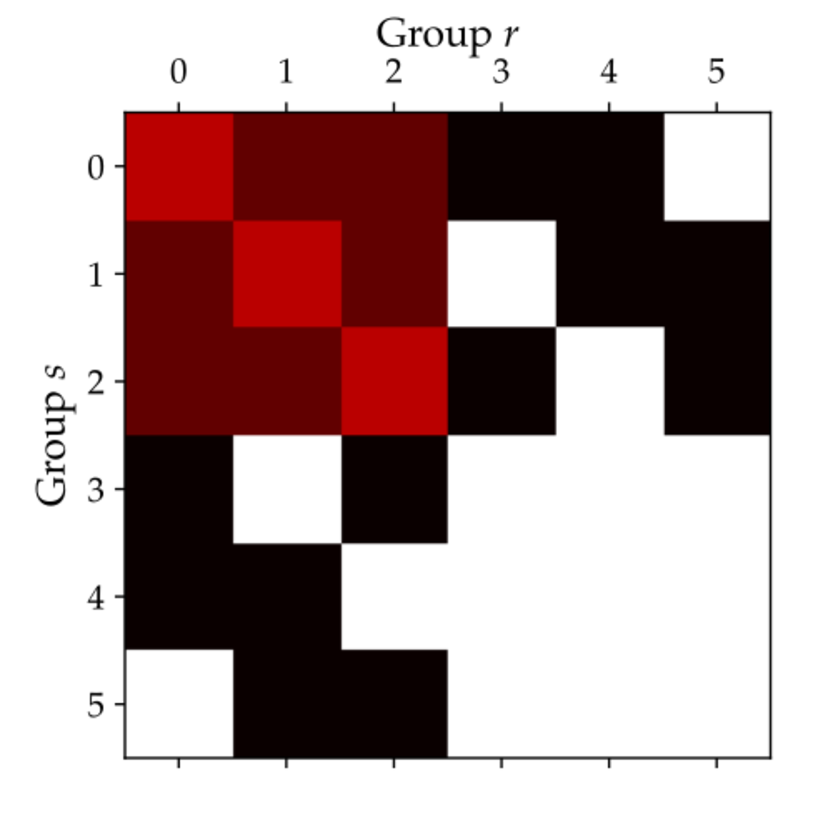
\includegraphics[width=0.3\linewidth]{pictures/topic/peixioto_ers.pdf}
  \caption{Example of an edge's matrix from~\cite{peixoto_graph-tool_2014}}
    \label{fig:hsbm-ers}
\end{figure}

It is useful to define a traditional entropy:
\begin{equation}\label{eq:hSBMentropyt}
  S_t=\frac{1}{2}\Sigma_{r,s} n_rn_sH\left(\frac{e_{rs}}{n_rn_s}\right)
\end{equation}
where $n_{r}$ is the number of nodes in groups $r$, $e_{rs}$ is the number of edges between nodes of group $r$ and nodes of group $s$, and $H(x)=-xln(x)-(1-x)ln(1-x)$. This entropy is equivalent to the micro-canonical entropy of a system with ${\Omega(A,\{n_r\})}$ accessible states $S_t=Ln\Omega$.

The algorithm uses a Markov Chain Monte Carlo to minimize this entropy. Made it simple, each step a node changes block and the new configuration is accepted if $S$ is decreased.

Note that~\ref{eq:hSBMentropyt} can be corrected taking care of degree distribution obtaining corrected entropy $S_c$
\begin{equation}
  S_c=-\Sigma_{r,s}\frac{e_{rs}}{2}-\Sigma_k
  N_kln(k!)-\frac{1}{2}\Sigma_{r,s}e_{rs}ln\left(\frac{e_{rs}}{e_re_s}\right)
\end{equation}

\paragraph{How to change group of a node?}\mbox{}\\
At each step according to~\cite{peixoto2014efficient} node $i$ can change group from $r$ to $s$ with a probability
\begin{equation}\label{eq:Prst}
  P(r\to s|t)=\frac{e_{ts}+\epsilon}{e_t+\epsilon B}
\end{equation}
where $j$ is a random neighbour of $i$: $j\in N_i$, $t\in\{b_j\}$ its block as defined in~\cite{peixoto2014efficient}. $\epsilon$ is a parameter that according to~\cite{peixoto2017nonparametric} has no significant impact in the algorithm, provided it is sufficiently small.
Equation~\ref{eq:Prst} can be rewritten as \[P(r\to s|t)=(1-R_t)\frac{e_{ts}}{e_t}+\frac{R_t}{B}\] defining $R_t=\frac{\epsilon B}{e_t + \epsilon B}$
This is done in four steps for each node $i$:
\begin{itemize}
  \item a node $j$ is chosen from $i$'s neighbours, the group of $j$ is called
  $t$
  \item a random group $s$ is selected
  \item move of node $i$ to group $s$ is accepted with probability $R_t$
  \item if $s$ is not accepted, a random edge $e$ is chosen from group $t$ and node $i$ is assigned to the endpoint of $e$ which is not in $t$
\end{itemize}
This steps mime probability~\ref{eq:Prst}; note that for $\epsilon\to\infty$ this gives a uniform probability.

To enchant the probability to find a minimum, a bounce of these moves is made, only the set of moves with the minimum $S$ is accepted.

\paragraph{How many blocks $B$?}\mbox{}\\
Note that the number of blocks $B$ is a free parameter and must be inferred as described in~\cite{peixoto2017nonparametric}. This implies a slight modification of the algorithm such that it became possible to admit the creation of  a new group.
When a group $s$ is chosen, the algorithm can now accept a \textbf{new group} and~\ref{eq:Prst} became
\begin{equation}\label{eq:PrstB1}
  P(r\to s)=\Sigma_t P(t|i)\frac{e_{ts}+\epsilon}{e_t+\epsilon (B+1)}
\end{equation}
being $P(t|i)=\Sigma_j\frac{A_{ij}\delta(b_j, t)}{k_i}$ the fraction of neighbours of $i$ belonging to group $t$, $e_t$ the number of edges in group $t$,
$k_i$ the degree, and $b_j$ groups.

Using this modification it is now possible to add new groups and $B$ is no longer a parameter.

\paragraph{How to find hierarchic layers?}\mbox{}\\
After the algorithm is run, one would to add a new hierarchic level, this is done considering the $B$ groups as nodes and repeating the process.
As done before a matrix of edges like~\ref{fig:hsbm-ers} is created, where edges are considered between groups of the previous layer.
The posterior probability became
\begin{equation}\label{eq:posteriorL}
  P(\{b_l\}|A)=\frac{P(A|\{b_l\})P(\{b_l\})}{P(A)}=\prod_l^L P(b_l|e_l,b_{l-1})
\end{equation}
where $l=0\dots L$ is the layer, $A$ the audience matrix, $b_i$ blocks. Note that $e_0=A$ and $B_L=1$.
Maximising~\ref{eq:posteriorL} gives the correct number of layers.

Adding a layer is done in 3 steps described in~\cite{peixoto2014hierarchic}:
\begin{itemize}
  \item[Resize] find $B_l\in[B_{l-1},B_{l+1}]$ by bisection
  \item[Insert] a layer l
  \item[Delete] $l$ and linking nodes from layer $l-1$ directly to groups of layer
  $l+1$
\end{itemize}
One marks initially all levels as not done and starts at the top level $l = L$~\cite{peixoto2014hierarchic}.
For the current level $l$, if it is marked done it is skipped and one moves to the level $l-1$. Otherwise, all three moves are attempted. If any of the moves succeeds in decreasing the description length $\Sigma$~\ref{eq:descriptionlenght}, one marks the levels $l-1$ and $l+1$ (if they exist) as not done, the level $l$ as done, and one proceeds (if possible) to the upper level $l+1$, and repeats the procedure. If no improvement is possible, the level $l$ is marked as done and one proceeds to the lower level $l-1$. If the lowest level $l=0$ is reached and cannot be improved, the algorithm ends.


\paragraph{Overlapping partitions}\mbox{}\\
As described in~\cite{peixoto2015model} one of the advantages of this approach is that it is possible to let a node belonging to multiple groups.
In this case $b_i$ becomes $\vec{b_i}$, with component $b_{ir}=1$ if node $i$ is in group $r$, $0$ otherwise. The number of $1$s in vector $\vec{b_i}$ is called
$d_i=|\vec{b_i}|$.

The probability of having a graph $G$ being generated from an adjacency matrix $A$ and a partition $\{\vec{b_i}\}$ is \[P(G|A,\{\vec{b_i}\})=\frac{1}{\Omega}\]
if $\Omega$ is the number of possible graphs. Entropy~\ref{eq:hSBMentropyt} is $S_t=Ln\Omega$. This corresponds to an augmented graph generated via a
non overlapping block model with $N'=\Sigma_r n_r>N$ nodes and the same adjacency matrix $A$.

First of all, it is necessary to sample the distribution of mixture sizes $P(\{n_d\})$ where $n_d$ is the number of nodes which mixture has got size $d$, $n_d\in[0,N]$ and $d\in[0,D]$ (typically $D=B$ and in the non-overlapping case $D=1$), this is done by sampling uniformly from \[P(\{n_d\}|B)=\left(\binom{D}{N}\right)^{-1}\] which is probability of having $n$ nodes whose mixture has size $d$. $\left(\binom{B}{N}\right)$ is the number of histograms with area $N$ and $B$ distinguishable bins. $B-1$ can be used instead of $B$ to avoid node with no group, in this case $d\in[1,B]$.

Given the mixture sizes, the distribution of node membership is sampled from \[P(\{d_i\}|\{n_d\})=\frac{\prod_{d} n_d!}{N!}\].

At this point for each set of nodes with $d_i=d$ it is necessary to sample $n_{\vec{b}}$; the number of nodes with a particular mixture $\vec{b}$. It is sampled from
\begin{equation}
  P(\{n_{\vec{b}}\}_d|n_d)=\left(\binom{\binom{D}{d}}{n_d}\right)^{-1},
\end{equation}
next all mixtures $\vec{b_i}$ of size $d$ must be sampled, they are given by
\begin{equation}
  P(\{\vec{b_i}\}_d|\{n_{\vec{b}}\}_d)=\frac{\prod_{|\vec{b_i}|=d} n_b!}{n_d!}
\end{equation}
the global posterior as defined in~\cite{peixoto2015model} is
\begin{equation}
  P(\{\vec{b_i}\}|B)=\left[\prod_{d=1}^B  P(\{\vec{b_i}\}_d|\{n_{\vec{b}}\}_d) P(\{n_{\vec{b}}\}_d|n_d)\right]P({d_i}|{n_d})P(n_d|B)
\end{equation}

At this time it is necessary to obtain the distribution of the edges between mixtures. Defined $e_r=\Sigma_s e_{rs}$ the number of half-edges labelled $r$, $m_r=\Sigma_{\vec{b}} b_r$ the number of mixtures containing group $r$ the algorithm samples the probability distribution of the edges count
\[P(\{e_{\vec{b}}\}|\{\vec{b_i}\}, A)=\prod_r\left(\binom{m_r}{e_r}\right)^{-1}\] and the labeled degree sequence $\{\vec{k_i}\}$ from \[P(\{\vec{k_i}\}_{\vec{b}}|\{e_{\vec{b}}\}, \{\vec{b_i}\})=\frac{\prod_k n_k^{\vec{b}}!}{n_{\vec{b}}!}\]
\begin{figure}[htb]
	\centering
	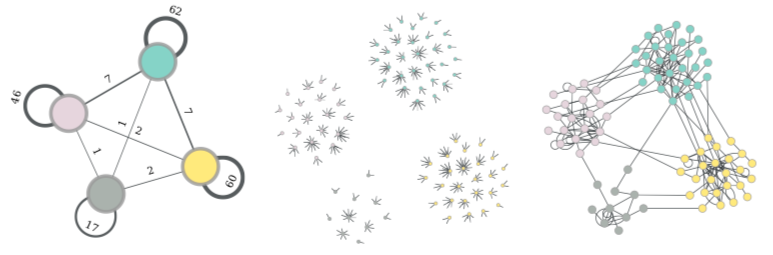
\includegraphics[width=0.8\linewidth]{pictures/topic/peixioto_passages.png}
	\caption{Illustration of the generative process of the microcanonical SBM. Given a partition of the
		nodes, the edge counts between groups are sampled (left), followed by the degrees of the nodes (center) and finally
		the network itself (right). From~\cite{Peixoto2017}.}
	\label{fig:hsbm-sum}
\end{figure}

\paragraph{Word documents separation}\mbox{}\\
Following what is done in~\cite{gerlach2018network}, the probability of a group $P(b_l)$ at a certain level $l$ is intended as the disjoint probability of group of words and group of documents.
\begin{equation}
  P(b_l)=P_w(b_l^w)P_d(b_l^d)
\end{equation}
Doing this let words and documents be separated by construction. Considering the process described above if two nodes are not connected at the beginning it is impossible that they end up in the same block. It is easily verified in~\cite{peixoto2014efficient} that this property is preserved and fully reflected in the final block structure.
